\newpage
{\bfseries ҒТАМР 61.43.29}

{\bfseries ЖАРЫЛЫС ЖҰМЫСТАРЫНДА ЭМУЛЬСИЯЛЫҚ ЖАРЫЛҒЫШ ЗАТТАРДЫ ҚОЛДАНУДЫҢ
ТИІМДІЛІГІН ТАЛДАУ}

{\bfseries Э.Қ. Қаржауова, Д.Д. Мейрам, Ж.Т. Нұртай, А.Ж. Хамит, С.Ж.
Қалыхбергенова}

Қ.Құлажанов атындағы Қазақ технология және бизнес университеті, Астана,
Қазақстан

Корреспондент-автор: karzhauova.81@mail.ru

Тау-кен массивтерін жару көмегімен бұзылуының дамуы тау-кен
кәсіпорындарында тікелей әзірленетін, құрамында жарылғыш компоненттері
жоқ ЖЗ-дың эволюциясымен байланысты.

Өнеркәсіптік ЖЗ-мен салыстырғанда эмульсиялық ЖЗ тиімдірек, бұл жоғары
зарядтау тығыздығына және соның салдарынан жарылыс энергиясының көлемдік
концентрациясының және ұңғыма зарядтарының жарылу жылдамдығының жоғары
мәндеріне байланысты. Нәтижесінде ЭЖЗ күшті тау жыныстары үшін қолайлы
кернеу толқындарының алдыңғы жағындағы қысымның жоғарылауымен ғана емес,
сонымен қатар, сұйық фазаның (эмульсияның) болуына байланысты оны ұзақ
уақыт бойы ұстап тұрады, бұл зарядтан алыстау кезінде ұсақтау
тиімділігін арттырады.

Эксперименттік зерттеулермен ANFO кешенінде ЭЖЗ қолданған кезде
біртектілікке қатысты аралас зарядтың жұмыс қабілеттілігін 15\%-ға
ұлғайту есебінен жоғары жиектері бар жағдайларда бұрғылау-жару
жұмыстарының тиімділігі жоғарылайтыны, кендер мен сыйымды жыныстар
шекарасының жылжуы 1,5...2,0 есе азаятыны, ЖЗ шығындарын 0,9\%-ға
төмендете отырып, тау массасының ұсақталу сапасы жақсаратыны дәлелденді;
жарылыс жұмыстарының ЭеҚЖ-мен кешенде ЭЖЗ қолдануға ауысуымен тау
жыныстарын ұсақтау сапасы үйіндідегі жарылған бөліктің орташа мөлшерінің
15,8\%-ға және ЖЗ шығындарының 0,8\%-ға төмендеуімен жақсарады.

{\bfseries Түйін сөздер:} эмульсиялық жарылғыш заттар, су-гельді
өнеркәсіптік жарылғыш заттар, жарылыс энергиясын реттеу, детонация
жылдамдығы, электрлік емес инициация жүйелері, түйіршікті аммиак
селитрасының сусымалы қоспасы, дизель отыны.

{\bfseries АНАЛИЗ ЭФФЕКТИВНОСТИ ПРИМЕНЕНИЯ ЭМУЛЬСИОННЫХ ВЗРЫВЧАТЫХ ВЕЩЕСТВ
ПРИ ВЗРЫВНЫХ РАБОТАХ}

{\bfseries Э.Қ. Қаржауова, Д.Д. Мейрам, Ж.Т. Нұртай, А.Ж. Хамит, С.Ж.
Қалыхбергенова}

Казахский университет технологии и бизнеса имени К.Кулажанова, Астана,
Казахстан,

e-mail: karzhauova.81@mail.ru

Прогресс во взрывном разрушении массивов горных пород связан с эволюцией
ВВ в направлении развития составов без взрывчатых компонентов,
изготовляемых непосредственно на горных предприятиях.

Эмульсионные ВВ по сравнению с промышленными являются более
эффективными, что обусловлено более высокой плотностью заряжания и, как
следствие, более высокими значениями объемной концентрации энергии
взрыва и скорости детонации скважинных зарядов. Вследствие этого, ЭВВ
характеризуются не только повышенным давлением на фронте волн
напряжений, приемлемым для крепких пород, но благодаря присутствию в
составе жидкой фазы (эмульсии), поддерживают его в течение более
длительного промежутка времени, что повышает эффективность дробления на
удалении от заряда.

Экспериментальными исследованиями доказано, что при применении ЭВВ в
комплексе с ANFO повышается эффективность буровзрывных работ в условиях
с высокими уступами за счет увеличения работоспособности
комбинированного заряда относительно однородного на 15\%, уменьшается в
1,5\ldots2,0 раза смещение границы руды и вмещающих пород, улучшается
качество дробления горной массы при одновременном снижении затрат на ВВ
на 0,9\%; с переходом взрывных работ на применение ЭВВ в комплексе с НСИ
качество дробления пород улучшается со снижением среднего размера
взорванного куска в развале на 15,8\% и затрат на ВВ на 0,8\%.

{\bfseries Ключевые слова:} эмульсионные взрывчатые вещества, водногелевые
промышленные взрывчатые вещества, регулирование энергией взрыва,
скорость детонации, неэлектрические системы инициирования, сыпучая смесь
гранулированной аммиачной селитры, дизельное топливо

{\bfseries ANALYSIS OF THE EFFECTIVENESS OF THE USE OF EMULSION EXPLOSIVES
IN BLASTING OPERATIONS}

{\bfseries E.K. Karzhauova, D.D. Meiram, Z.T. Nurtai, A.Zh. Hamit, S.Zh.
Kalyhbergenova}

Kazakh technology named after K. Kulajanov and a business university,
Astana, Kazakhstan,

e-mail: karzhauova.81@mail.ru

Progress in the explosive destruction of rock massifs is associated with
the evolution of explosives in the direction of the development of
compositions without explosive components manufactured directly at
mining enterprises, equipment and technology for charging wells.

Emulsion explosives are more effective compared to industrial
explosives, which is due to a higher charging density and, as a result,
higher values of the volumetric concentration of explosion energy and
the detonation rate of borehole charges. As a result, EVs are
characterized not only by increased pressure at the front of stress
waves, acceptable for strong rocks, but due to the presence of a liquid
phase (emulsion) in the composition, they maintain it for a longer
period of time, which increases the crushing efficiency at a distance
from the charge.

Experimental studies have proved that when using EVV in combination with
ANFO, the efficiency of drilling and blasting operations in conditions
with high ledges increases by increasing the efficiency of the combined
charge relatively homogeneous by 15\%, the displacement of the ore
boundary and the host rocks decreases by 1.5...2.0 times, the quality of
crushing rock mass improves while reducing the cost of explosives by
0.9\%; with the transition of blasting operations to the use of EVV in
combination with NSI, the quality of rock crushing improves with a
decrease in the average size of the exploded piece in the collapse by
15.8\% and the cost of explosives by 0.8\%.

{\bfseries Key words:} emulsion explosives, water-gel industrial
explosives, regulation of explosion energy, detonation rate,
non-electric initiation systems, bulk mixture of granular ammonium
nitrate, diesel fuel

{\bfseries Кіріспе.} Соңғы екі онжылдықта пайда болған жарылыс жұмыстарының
экономикалық тиімділігі мен олардың қауіпсіздігінің артуы қарапайым
құрамдағы жарылғыш заттардың және құрамында суы бар жарылғыш заттардың
пайда болуымен байланысты.

Бұл қатарда маңызды орынды эмульсиялық жарылғыш заттар алады, олардың
негізгі артықшылықтары өндіріс пен пайдалану қауіпсіздігінің ең жоғары
деңгейі, тиеу процесін толық механикаландыру мүмкіндігі, энергетикалық
сипаттамаларды реттеу, сонымен қатар, шикізат құны қол жетімділігі және
төмен болуы болып табылады.

Өзектілігі. Қазіргі уақытта ашық тау-кен жұмыстарын жүргізу кезінде аршу
жұмыстарының күрт артта қалуына байланысты және болашақта тау-кен
жұмыстарының одан әрі дамуына байланысты пайдалы қазбаларды игеру үшін
тау-кен жоталарын дайындау жағдайы өршігіп кетті. Сондықтан, тау-кен
өнеркәсібінде өте маңызды мәселені шешу мәселесі туындады: аршу
жұмыстарын жүргізуді едәуір күшейту.

Мақсаты: бұрғылау-жару жұмыстарының тиімділігін арттыруды қамтамасыз
ететін эмульсиялық жарылғыш заттардың параметрлерін негіздеу.

{\bfseries Материалдар мен әдістер.} Бұл эмульсиялық жарылғыш заттардың
құрамында жеке жарылғыш заттар жоқ, сондықтан қауіпті жүктерді
тасымалдау мен сақтаумен байланысты проблемалар жойылады. Дегенмен,
абсолютті қауіпсіз жарылғыш заттар жоқ екенін және тотықтырғыш пен
отынның кез келген қоспасы жарылғыш болуы мүмкін екенін және оны өңдеу
кезіндегі нақты қауіптілік дәрежесі көптеген факторларға байланысты
екенін есте ұстаған жөн {[}1{]}.

Жарылғыш заттардың бұл түрінің айқын тартымдылығы көптеген тау-кен
кәсіпорындарында, әсіресе ірі кәсіпорындарда оларды өндіру және
пайдалану үшін кешендердің белсенді құрылысына әкелді.

Эмульсиялық жарылғыш заттардың маңызды ерекшеліктерінің бірі эмульгатор
зарядының көлемдік энергиясының концентрациясын мәжбүрлеп реттемей, оның
бастапқы импульске сезімталдығына қол жеткізе отырып және тығыздықты
өзгерту арқылы қол жеткізілетін детонацияның критикалық диаметрін
өзгертпестен, композицияның өзі жарылғыш зат болып табылмайды.
Эмульгаторды оған химиялық агенттерді (химиялық газ генерациясы) немесе
механикалық қоспаларды (шыны сферасы, перлит, тығыздығы төмен
полимерлер) енгізу арқылы қол жеткізіледі.

Сонымен қатар, эмульсия эмульсияларының құрамында түйіршіктелген
(кеуекті) аммоний нитраты немесе ANFO типті қоспалар болуы мүмкін, бұл
жағдайда эмульсияның пайызы 30-дан 70\%-ға дейін өзгеруі мүмкін. Осы
ерекшелігіне байланысты жарылғыш заттар стандартты өнеркәсіптік жарылғыш
заттармен салыстырғанда өндіру және пайдалану үшін ең қауіпсіз болып
табылады. Жалпы алғанда, олар тотықтырғыштардың сулы ерітіндісі
(негізінен аммоний, натрий, кальций нитраттары) дисперсті фаза болып
табылатын және дисперсиялық орта сұйық немесе балқытылған отынмен
(негізінен мұнай өңдеу өнімдері) түзілетін әдеттегі жоғары концентрлі
эмульсияны білдіреді {[}2{]}.

Физикалық химиядағы эмульсияның бұл түрі кері деп жіктеледі және
«мұнайдағы су» деп белгіленеді. Мұндай эмульсияларда сулы фазаның әрбір
тамшысы суда ерімейтін органикалық заттардың қабығында болады.
Эмульсияның жалпы оң қасиеттерін (тотықтырғыштың өте аз өлшемдері бар
үлкен аралық беті) пайдалану тотықтырғыштың отынмен тығыз байланысын
және олардың жарылғыш масса бойынша біртекті таралуын алуға мүмкіндік
береді, бұл композицияларға сан береді. Компоненттерді араластырудың
әдеттегі механикалық әдістерімен қол жеткізуге болмайтын оң қасиеттер.
Осылайша, эмульсиялық жарылғыш заттардың көмегімен жарылғыш заттардың
детонацияға жоғары сезімталдығымен бір мезгілде қауіпсіз қолдануға
болатын рецептураларын алу мүмкін болды. Өлшемдері 1-ден 50 мкм-ге
дейінгі ең кішкентай тотықтырғыш бөлшектердегі отынның микроскопиялық
пленкасы бар композицияның алынған эмульсиялық құрылымы (1-сурет)
бұрғылаудан кейін тиеу технологиясын қолдана отырып, оларды пайдалану
мүмкіндігімен ПЖЗ (пластикалық жарылғыш заттар) жоғары суға төзімділігін
қамтамасыз етеді. Эмульсиялық жарылғыш заттардың экологиялық тазалығы
ерекше назар аударуды қажет етеді, бұл жарылыс қаупін өзгерту кезінде
де, жарылыс алдында тау жыныстарымен және жер асты суларымен жанасқанда
да қамтамасыз етіледі {[}3{]}. Эмульсиялық жарылғыш заттарды қолдану
тәжірибесі жарылғыш заттардың басқа кластарына қарағанда бірқатар
артықшылықтарды көрсетті:

-- механикалық және термиялық әсерлерге (соққы, үйкеліс, жылу, өрт,
оқтың өтуі және т.б.) қатысты жоғары қауіпсіздік;

-- 0,5-тен 1,5 г/см\textsuperscript{3}-ке дейінгі жұмыс тығыздығының кең
диапазоны бар жарылғыш сипаттамаларды реттеу мүмкіндігі;

-- ағынды суларда және үлкен тереңдікте сақталған жоғары суға
төзімділік;

-- стандартты праймерден және қажет болған жағдайда тек аралық
детонатордан іске қосылған кездегі селективті сезімталдық;

-- тозаңданудың, электролиздің, компоненттердің экссудациясының және улы
материалдармен жанасуының болмауы;

-- жарылыс кезінде аз уыттылықпен газдың шығуын қамтамасыз ететін
жүйенің оттегі балансының нөлге жақын, жарылыс жұмыстарын толық
механикаландыру;

-- әртүрлі қоспаларды енгізе отырып, матрицалық эмульсия негізінде
құрама және аралас композициялар құру мүмкіндігі;

-- эмульсиялардың реологиялық қасиеттерін әр түрлі стандартты өлшемдегі
картридждер түрінде шығаруға мүмкіндік беретін, пайдалану орнында толық
көлденең қимасына дейін толтыра отырып дайындалу;

-- пайдаланудың жоғары техникалық-экономикалық тиімділігі бар жарылғыш
заттарды алуға мүмкіндік беретін қолжетімді және арзан шикізат базасы.
% TODO
%\begin{figure}[H]
%	\centering
%	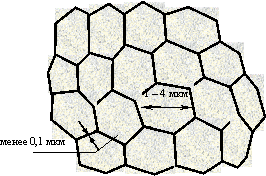
\includegraphics[width=0.8\textwidth]{assets/68}
%	\caption*{}
%\end{figure}

%\begin{figure}[H]
%	\centering
%	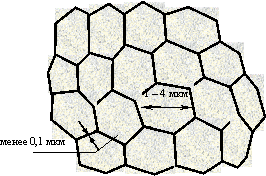
\includegraphics[width=0.8\textwidth]{assets/68}
%	\caption*{}
%\end{figure}
%\emph{май қабаты}
%\begin{figure}[H]
%	\centering
%	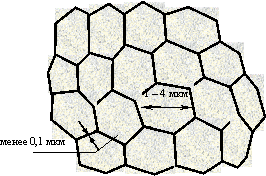
\includegraphics[width=0.8\textwidth]{assets/68}
%	\caption*{}
%\end{figure}\emph{тотығу
%бөлшектері}

{\bfseries 1-сурет - Эмульсия құрылымы}

\emph{Эмульсиялық жарылғыш заттардың қасиеттері}

{\bfseries 1-кесте - Эмульсиялық жарылғыш заттардың негізгі сипаттамалары}

\begin{longtable}[]{@{}
  >{\raggedright\arraybackslash}p{(\columnwidth - 10\tabcolsep) * \real{0.1630}}
  >{\raggedright\arraybackslash}p{(\columnwidth - 10\tabcolsep) * \real{0.1522}}
  >{\raggedright\arraybackslash}p{(\columnwidth - 10\tabcolsep) * \real{0.2132}}
  >{\raggedright\arraybackslash}p{(\columnwidth - 10\tabcolsep) * \real{0.1522}}
  >{\raggedright\arraybackslash}p{(\columnwidth - 10\tabcolsep) * \real{0.1920}}
  >{\raggedright\arraybackslash}p{(\columnwidth - 10\tabcolsep) * \real{0.1275}}@{}}
\toprule\noalign{}
\begin{minipage}[b]{\linewidth}\raggedright
Жарылғыш заттар
\end{minipage} & \begin{minipage}[b]{\linewidth}\raggedright
Жарылыс жылуы, ккал/кг
\end{minipage} & \begin{minipage}[b]{\linewidth}\raggedright
Энергия концентрациясы, ккал/дм\textsuperscript{3}
\end{minipage} & \begin{minipage}[b]{\linewidth}\raggedright
Тығыздығы жүктелген, кг/м\textsuperscript{3}
\end{minipage} & \begin{minipage}[b]{\linewidth}\raggedright
Детонация жылдамдығы, км/с
\end{minipage} & \begin{minipage}[b]{\linewidth}\raggedright
Газдың зияндылығы, л/кг
\end{minipage} \\
\midrule\noalign{}
\endhead
\bottomrule\noalign{}
\endlastfoot
Гранулотол & 980 & 980 & 1000 & 5,0-5,2 & 275 \\
Игданит & 920 & 820 & 900 & 2,2-2,7 & 45 \\
Порэмит 1 & 689-726 & 861-908 & 1250 & 4,9-5,2 & 11,8-12,2 \\
Порэмит М & & & & 4,8-5,3 & 42-54 \\
Гранэмит 50/50 & 835 & 1170 & 1400 & 4,8-5,2 & 36 \\
\end{longtable}

Тұрмыстық эмульсиялық жарылғыш заттардың (поремит) негізгі техникалық
сипаттамалары 1-кестеде берілген, салыстыру үшін стандартты жарылғыш
заттардың -- гранулотол мен игданиттің сипаттамалары келтірілген
{[}4{]}.

1-кестеде тотықтырғыш бөлігінің құрамы, қолданылатын отын-энергетикалық
қоспалары бойынша ерекшеленетін поремиттердің екі түрі көрсетілген.
Әртүрлі маркадағы поремиттер жарылу жылуы бойынша (салмағы бойынша)
гранулотолдан айтарлықтай төмен, алайда, ұңғымаларды поремиттермен тиеу
тығыздығының жоғарылауын ескере отырып, энергия концентрациясы
гранулотолдың қуат деңгейіне жақындайды. Жүктеме тығыздығын 1350
кг/м\textsuperscript{3} дейін арттыруға және гранулотол деңгейінде
поремиттік энергия концентрациясын алуға болады. Бұл жарылғыш заттарды
судың кез келген дәрежесі бар орташа қатты жыныстарды жару үшін тиімді
пайдалануға болады. Күшті және өте берік тау жыныстары үшін құрамында
энергетикалық қоспа -- алюминий бар қуатты эмульсиялық жарылғыш заттарды
қолдану ұсынылады. Қуаттылығы бойынша алюминиизацияланған жарылғыш
заттар (жоғары тығыздығын ескере отырып) шихтадағы энергия
концентрациясы бойынша гранулотолдан айтарлықтай асып түседі, сондықтан
оларды кез келген беріктіктегі және су құрамындағы тау жыныстарында жару
үшін қолдануға болады.

Дегенмен, таза эмульсиялық жарылғыш заттардың, әсіресе алюминий
қоспалары бар, жоғары құны бар, сондықтан гранемиттер, эмульсия
негізіндегі аралас жарылғыш заттар және түйіршіктелген аммоний нитраты
немесе AС-ДT 30/70 қатынасында (70\% эмульсия, қалғаны селитра немесе
AС-ДT) {[}5{]}.

Зарядтау тығыздығы кг/м3 гранемиттер қуаты жағынан гранулотолдан біршама
жоғары және оның орнына жарылыс жұмыстарында тиімді пайдалануға болады.
Эмульсиялық жарылғыш заттар детонация жылдамдығы бойынша гранулотол
деңгейінде және онымен салыстырғанда газ зияндылығы айтарлықтай төмен.

2-кестеде картриджді эмульсиялық жарылғыш заттардың негізгі
сипаттамалары көрсетілген, салыстыру үшін аммонит 6ЖВ сипаттамалары
берілген. Патронды эмульсиялық жарылғыш заттардың жарамдылық мерзімі 6
ай.

{\bfseries 2-кесте - Патрондық эмульсиялық жарылғыш заттардың негізгі
сипаттамалары}

\begin{longtable}[]{@{}
  >{\raggedright\arraybackslash}p{(\columnwidth - 10\tabcolsep) * \real{0.2341}}
  >{\raggedright\arraybackslash}p{(\columnwidth - 10\tabcolsep) * \real{0.1527}}
  >{\raggedright\arraybackslash}p{(\columnwidth - 10\tabcolsep) * \real{0.1221}}
  >{\raggedright\arraybackslash}p{(\columnwidth - 10\tabcolsep) * \real{0.1731}}
  >{\raggedright\arraybackslash}p{(\columnwidth - 10\tabcolsep) * \real{0.1527}}
  >{\raggedright\arraybackslash}p{(\columnwidth - 10\tabcolsep) * \real{0.1653}}@{}}
\toprule\noalign{}
\begin{minipage}[b]{\linewidth}\raggedright
Жарылғыш заттар
\end{minipage} & \begin{minipage}[b]{\linewidth}\raggedright
Патрон диаметры, мм
\end{minipage} & \begin{minipage}[b]{\linewidth}\raggedright
Жарылыс жылуы, ккал/кг
\end{minipage} & \begin{minipage}[b]{\linewidth}\raggedright
Патрондағы ЖЗ массасы, кг
\end{minipage} & \begin{minipage}[b]{\linewidth}\raggedright
Патрондағы ЖЗ тығыздығы, кг/м\textsuperscript{3}
\end{minipage} & \begin{minipage}[b]{\linewidth}\raggedright
Детонация жылдамдығы, км/с
\end{minipage} \\
\midrule\noalign{}
\endhead
\bottomrule\noalign{}
\endlastfoot
Аммонит 6ЖВ & 32; 36; 90 & 1030 & 0,2\ldots3,5 & 1,00 - 1,10 & 3,6 -
4,8 \\
Порэмит ПГА, I & 45; 60; 90 & 1025 & 1,0\ldots4,3 & 1,40 - 1,60 & 5,0 -
6,0 \\
Порэмит ПГ-4А & 32; 36; 45 & 875 & 0,2\ldots0,5 & 1,10 - 1,25 & 3,6 -
4,4 \\
\end{longtable}

Құрамына қарай эмульгаторларды екі негізгі топқа бөлуге болады:
сенсибилизацияланған эмульсия және сенсибилизацияланған (немесе
сенсибилизацияланбаған) эмульсияның аммоний селитрасымен немесе AS+DT
(дизельдік отынмен майланған аммоний нитраты) қоспалары, олардың
саудалық атаулары әртүрлі елдер әртүрлі, бірақ негізінен «Эмуландар»,
«Гранемиттер», «Нобеландар» және т.б. типтерге біріктірілуі мүмкін. Ең
қарапайым класқа жататын қазіргі заманғы эмульсиялық жарылғыш заттар
(ЭМБ) өндіру мен пайдалану үшін ірі тау-кен кәсіпорындары үшін ғана
мүмкін күрделі және қымбат технологияны қажет етеді.

Осыған байланысты тау-кен өндірісінде әзірленген және қолданылатын
жарылғыш заттардың ассортименті әртүрлі болып қалуда.

Келесі топтарды бөлуге болады: құрамында тротил бар, су өткізбейтін
(аммониттер, комбизарлар және т.б.); құрамында тротил бар су
(акватолдар, ифзаниттер, карбатолдар және т.б.); түйіршікті тротил бар
су өткізбейтін (гранулотол, граммониттер, тротил U); түйіршікті
тротилсіз (игданиттер, коалиттер, гранулиттер және т.б.); эмульсия
(поремиттер, сибириттер, тован және т.б.); қорғаныш (карбониттер,
аммониттер); конверсия (гранипоралар, жоғары жарылғыш заттар) {[}6{]}.

Соңғы онжылдықта әртүрлі параметрлері бар жарылғыш заттардың 20-ға жуық
құрамы ұсынылды; Зауытта да, жарылыс алаңдарында да өндірілетін
акватолдардың, гранулотолдардың, карбониттердің және т.б. 6-8 құрам.
Эмульсиялық жарылғыш заттар есебінен жарылғыш заттарды тұтынудың артуы
байқалды, оның ішінде су өткізбейтін эмульсиялық композицияларға
40-50\%-ға дейін игданит қосу, олардың суға төзімділігін сақтай отырып,
эмульсиялық жарылғыш заттардың тиімділігін арттыру.

Стационарлық модульдік кешендегі эмульсиялық жарылғыш заттардың
өнеркәсіптік өндірісінің құрылымдық схемасы келесі технологиялық
кезеңдерді қамтиды: шикізатты дайындау; тотықтырғыштардың (селитра) және
май фазасының (минералды май, парафин және эмульгатор қоспасы)
ерітіндісін дайындау; эмульсия (матрицалық дайындау) -- арнайы
динамикалық араластырғышта тотықтырғыш және май ерітінділерін араластыру
арқылы эмульсия түзу; аммиак селитрасын (АС) дизельдік отынмен (ДО)
араластыру, матрицалық эмульсияны АЗМ бункеріне қабылдау; АЗМ
ұңғымаларына эмульсиялық жарылғыш заттарды тиеу: эмульсияларды
сенсибилизациялау -- газ түзетін қоспаларды (ГТҚ) қосу {[}7{]}.

Эмульсиялық жарылғыш заттарды өндіруде эмульсиялық матрицаны (эмульсия),
содан кейін аралас эмульсиялық жарылғышты құрайтын компоненттер
қолданылады (3-кесте).

{\bfseries 3-кесте - Эмульсиялық жарылғыш заттарды өндіруге арналған
компоненттер}

\begin{longtable}[]{@{}
  >{\raggedright\arraybackslash}p{(\columnwidth - 8\tabcolsep) * \real{0.2729}}
  >{\raggedright\arraybackslash}p{(\columnwidth - 8\tabcolsep) * \real{0.1225}}
  >{\raggedright\arraybackslash}p{(\columnwidth - 8\tabcolsep) * \real{0.1596}}
  >{\raggedright\arraybackslash}p{(\columnwidth - 8\tabcolsep) * \real{0.1127}}
  >{\raggedright\arraybackslash}p{(\columnwidth - 8\tabcolsep) * \real{0.3324}}@{}}
\toprule\noalign{}
\begin{minipage}[b]{\linewidth}\raggedright
Компоненттер
\end{minipage} & \begin{minipage}[b]{\linewidth}\raggedright
Химиялық формуласы
\end{minipage} & \begin{minipage}[b]{\linewidth}\raggedright
Эмульсия құрамындағы үлес, \%
\end{minipage} & \begin{minipage}[b]{\linewidth}\raggedright
Сатылу түрі
\end{minipage} & \begin{minipage}[b]{\linewidth}\raggedright
Қолданылуы
\end{minipage} \\
\midrule\noalign{}
\endhead
\bottomrule\noalign{}
\endlastfoot
1. Аммоний нитратының ыстық ерітіндісі (82 \%) &
NH\textsubscript{4}NO\textsubscript{3} & 87,8 & сұйық &
\multirow{5}{=}{Тотықтырғыш ерітіндіде} \\
2. Натрий нитраты & NaNO\textsubscript{3} & 4,0 & қатты \\
3. Сірке қышқылы (60

\%) & C\textsubscript{2}H\textsubscript{4}O\textsubscript{3} & 0,4 &
сұйық \\
4. Тиомочевина & (H\textsubscript{2}N)\textsubscript{2}CS & 0,25 &
қатты \\
5. Күйдіргіш натр & NaOH & 0,15 & қатты \\
6. Минерал майы & Mineral Oil & 5,9 & сұйық & \multirow{2}{=}{Майлы
ерітінідіде} \\
7. Эмульгатор DN серии

2000 & ПАВ & 1,2 & сұйық \\
8. Натрий нитраты & NaNO\textsubscript{2} & 0,3 & қатты & ГГД \\
9. Түйіршіктелген аммоний нитраты & NH4NO3 & 94\% қоспа құрамында АС+ДТ
& қатты & \multirow{2}{=}{АС+ДТ қоспасын қалыптастыру үшін} \\
10. Дизель отыны & - & 6\% қоспа құрамында АС+ДТ & сұйық \\
\end{longtable}

{\bfseries Нәтижелер мен талқылау}. Осылайша, тау-кен массивтерін жарылғыш
жолмен жоюдағы ілгерілеу жарылғыш заттардың тікелей тау-кен
кәсіпорындарында өндірілетін жарылғыш компоненттері жоқ композицияларды
әзірлеуге, ұңғымаларды тиеуге арналған жабдықтар мен технологиялардың
эволюциясымен байланысты.

Сонымен қатар, жарылғыш жарылғыш заттардың тағы бір өте маңызды
артықшылығы бар: олар жарылыс алаңдарында дайындалады, нәтижесінде
жарылғыш заттарды тасымалдау шығындары айтарлықтай төмендейді және
олармен жұмыс істеу кезінде қауіпсіздік артады.

Эмульсиялық жарылғыш заттар негізінен тамшы түрінде дисперстік фазаны
білдіретін бейорганикалық тотықтырғыштың сулы ерітіндісінен және
үздіксіз фаза болып табылатын сұйық отыннан тұрады.

Алғашқы жарылғыш заттардың құрамында аммоний нитраттарының, перхлораттар
мен хлораттардың, сілтілі металдардың және сирек жер элементтерінің
тотықтырғыш ерітінділерінің ерітінділері болды. Көбінесе аммоний нитраты
жеке немесе басқа нитраттармен қоспада қолданылады. Эмульсиялық жарылғыш
заттардың жарылғыш сипаттамалары олардың газдануын өзгерту арқылы
өзгертілді {[}8{]}.

Жарылғыш зарядтардың алғашқы пилоттық жарылыстары 80-жылдардың аяғында
жүзеге асырылды және әдетте көңіл қуантарлық нәтижелер берді.

Эмульсиялық жарылғыш заттарды өндірудегі басты ерекшелігі эмульсия
матрицасында «ыстық нүктелердің» пайда болуы болып табылады, олар іске
қосылған кезде эмульсиялық жарылғыш заттардың жарылу орталығына
айналады. Қажетті сезімталдықты қамтамасыз ету үшін әзірленген
эмульсиялық композицияларға қуыс шыны микросфералар, кеуекті аммоний
нитраты және т.б. түріндегі әртүрлі сенсибилизаторлар («ыстық нүктелер»)
енгізілді.

90-жылдары эмульсияны салқындату кезінде натрий нитритінің
тиокарбамидпен әрекеттесуі кезінде химиялық жолмен түзілген азоттық
микрокөпіршіктермен эмульсия жарылғыш заттардың сенсибилизациясын
қамтамасыз ету мүмкін болды. Бұл кезде ең арзан бірінші жарылғыш заттар
пайда болды. Карьерлерде тау жыныстарын жару кезінде қолданылған
поремиттер.

Карьерлерде газ түзетін қоспалары бар жарылғыш заттарды қолдану арқылы
тәжірибелік-өндірістік және өнеркәсіптік жарылыс жұмыстарын жүргізу
жарылыс жұмыстарына кететін шығынды айтарлықтай төмендетуге және олардың
өндірістік қабілеттілігін арттыруға мүмкіндік берді.

Келесі жарылғыш заттар қолданылды: ANFO, Rioflex және Nitronit P

1. ANFO (ANFO) -- жарылғыш, құрғақ ұңғымаларға арналған оттегінің
теңдестірілген құрамы бар түйіршіктелген аммоний селитрасы мен дизельдік
отынның (ADF) түйіршікті қоспасы.

\emph{Қолдану}

ANFO бастапқыда құрғақ және іске қосылғанға дейін құрғақ болып қалатын
ұңғымаларда қолданылады. ANFO тау-кен өндірісінде, карьерде және жалпы
жарылыс жұмыстарында заряд бағанасы ретінде пайдаланылуы мүмкін.

ANFO-ны дұрыс қолданбау жарылыс газдарының жоғарылауына әкелуі мүмкін.

АНФО сульфидтері бар реактивті жыныстарда қолданылмайды.

\emph{Негізгі артықшылықтар}

• ANFO зарядтауға оңай және ұңғыманы толығымен толтырып, максималды
энергия шығаруды қамтамасыз етеді.

• Тұрақты жоғары сапа жарылыс сенімділігін қамтамасыз етеді.

• Үлкен жарылыстар үшін жоғары өнімділік.

2. «Rioflex» су-гельді өндірістік жарылғыш зат (TU
7276-011-58472318-2005) араластырғыш-зарядтау машинасымен ұңғымаларды
тиеу процесінде қолдану орнында MAXAM компаниясының рецептісі бойынша
дайындалған. Қоршаған орта температурасының -50°С-тан +50°C -ге дейінгі
диапазонында ұңғымаларды зарядтау әдісін қолдана отырып, М.М.
Протодьяконов шкаласы бойынша беріктік коэффициенті 20-ға дейінгі құрғақ
және су басқан тау жыныстарын жару кезінде жер бетіндегі жару
жұмыстарына арналған.

Rioflex жарылғыш заттар технологиясының соңғы жетістігін білдіреді және
жарылғыш емес ретінде тасымалданады, жарылғыш заттың өзі тұтынушы
орнында зарядтау және араластыру машинасында тікелей өндіріледі.

Rioflex-тің жарылғыш заттардың басқа түрлерінен артықшылығы:

- су басқан ұңғымаларды зарядтау кезінде суды жер бетіне шығару
мүмкіндігі;

- жарылғыш заттардың зарядталған массасы мен тығыздығын бақылау;

- ағын су болған жағдайда да суға жақсы төзімділік;

- жарылыс энергиясын және детонация жылдамдығын тығыздықты өзгерту
арқылы реттеу;

- жарылыстан жарылысқа дейінгі жұмыстың дәйекті және біркелкі сапасы.

- өнімді механикалық кернеуге ұшырату мүмкіндігі, яғни араластыру,
айдау, шнектің көмегімен беру.

Бұл өнімнің жоғарыда аталған барлық артықшылықтары тұтынушыға тау
жынысының сипаттамаларына және жарылған массаның қажетті профиліне жақсы
сәйкес келу үшін ұсақтау энергиясы мен тау жыныстарының сапасы
арасындағы қажетті теңгерімді таңдауға мүмкіндік береді {[}9{]}.

\emph{Картриджді жарылғыш заттар Nitronit P}

Капсула-сезімтал картридж негізіндегі жарылғыш заттар Nitronit-P
өнеркәсіптік жарылғыш заттардың ұңғымалары мен ұңғымаларын зарядтауды
бастау үшін тірі оқ-дәрі ретінде жарылыс жұмыстарында пайдалануға
арналған.

Олар габаритті емес материалдарды ұсақтау үшін үстеме шығындар ретінде
пайдаланылуы мүмкін.

Сонымен қатар, олар эмульсиялық жарылғыш заттармен қосылып суға төзімді
күшті жарылғыш зарядтар түзеді және суға төзімді емес жарылғыш заттармен
қосылып ұңғымалардың суарылатын бөлігінде жарылғыш зарядтар түзе алады.

Олар жер бетінде, жерасты шахталарында және газ немесе шаң әсерінен
қауіпті емес шахталарда қолданылады. Оларды пайдалану тау-кен
өндірісіндегі бұрғылау-жару жұмыстарының тиімділігін арттыруға мүмкіндік
берді (4-кесте).

{\bfseries 4-кесте - Техникалық сипаттамалары Nitronit P}

\begin{longtable}[]{@{}
  >{\raggedright\arraybackslash}p{(\columnwidth - 2\tabcolsep) * \real{0.5000}}
  >{\raggedright\arraybackslash}p{(\columnwidth - 2\tabcolsep) * \real{0.5000}}@{}}
\toprule\noalign{}
\begin{minipage}[b]{\linewidth}\raggedright
Диаметрі
\end{minipage} & \begin{minipage}[b]{\linewidth}\raggedright
25-тен 90 мм дейін
\end{minipage} \\
\midrule\noalign{}
\endhead
\bottomrule\noalign{}
\endlastfoot
Салмағы (диаметрге байланысты) & 0,15-тен 3,5 кг дейін \\
Ашық зарядтың жарылу жылдамдығы (диаметріне байланысты) & 5200-ден 5600
м/с дейін \\
Оттекті баланс & -1,7 \% \\
Патрондағы эмульсиялық жарылғыш заттың орташа тығыздығы & 1,1-ден 1,25
г/см³ дейін \\
15 м тереңдікке дейін суға төзімді & 100 \% \\
Жарылыс жылуы бойынша тротил эквиваленті & 0,74 \\
Қолдану температурасының диапазоны & −30ºC-тен +55ºC \\
\end{longtable}

Сондай-ақ, тау-кен өнеркәсібінде жарылыс жұмыстарын жүргізу кезінде
жарылғыш заттарды іске қосу құралдары қолданылады.

Бастау құралдары жарылғыш зарядқа бастапқы импульстің берілуін және оның
жарылуын қамтамасыз ету үшін қажет. Іске қосу құралдарын өндіруде
жарылғыш заттардың екі шартты тобы қолданылады: бастапқы және қайталама.
Біріншісіне сынап фульминаты, қорғасын азиді, тенерес сияқты
сезімталдығы жоғары заттар жатады. Сезімталдығы аз екінші топқа тетрил,
гексоген, ПЭТН жатады.

Зерттеу барысында Rionel электрлік емес инициация жүйелері қолданылды.
Rionel электрлік емес инициация жүйелері жер бетіндегі жарылыс жұмыстары
кезінде де, жер асты жағдайында да өнеркәсіптік жарылғыш зарядтарды
белсендіру үшін қолданылады. Жүйелерді пайдалану кезінде қоршаған орта
температурасы --50-ден +85 ° C-қа дейін болуы мүмкін. Rionel электрлік
емес жүйелерінің төрт негізгі өнімі шығарылады: MS, LP, X, DDX. MS --
0-750 мс диапазонында баяулатудың 21-сериясының детонаторларын
пайдаланатын миллисекундтық қатар.

Rionel LP сериялары жер асты және туннельдік қосымшалар үшін
пайдаланылатын 0-9000 мс ұзағырақ баяулау кезеңіне ие. X сериясы үстіңгі
монтаждау үшін пайдаланылады және 9-дан 150 мс аралығындағы жеті
номиналды жауап беру уақыты бар. DDX -- MS және X серияларының
параметрлерін біріктіретін қос баяулау сериясы.

Жалпы алғанда, Rionel жүйелері қауіпсіздіктің жоғары дәрежесіне және
жарылысты бақылаудың жоғары деңгейіне ие. Жүйелер пайдалануда сенімді,
біріктірілуі мүмкін және жарылғыш заттардың барлық түрлерімен
пайдалануға болады. Оларды пайдалану кезінде жарылғыш желінің бұзылуы
жойылады және ұңғымалардың зарядтарының «төменгі» бастамасы тиімді
қолданылады. Бұл жүйелердің қоршаған ортаға нөлдік дерлік зиянды әсері
де өзекті болып табылады (5-кесте).

{\bfseries 5-кесте -- Толқын бағыттағыштардың түрлері}

\begin{longtable}[]{@{}
  >{\raggedright\arraybackslash}p{(\columnwidth - 2\tabcolsep) * \real{0.5047}}
  >{\raggedright\arraybackslash}p{(\columnwidth - 2\tabcolsep) * \real{0.4953}}@{}}
\toprule\noalign{}
\begin{minipage}[b]{\linewidth}\raggedright
DDX
\end{minipage} & \begin{minipage}[b]{\linewidth}\raggedright
X
\end{minipage} \\
\midrule\noalign{}
\endhead
\bottomrule\noalign{}
\endlastfoot
Rionel DDX 25/500 6м & Rionel X 17м/с 6м \\
Rionel DDX 42/500 12м & Rionel X 25м/с 7.8м \\
Rionel DDX 25/500 12м & Rionel X 17м/с 7.8м \\
Rionel DDX 42/500 15м & Rionel X 25м/с 9м \\
Rionel DDX 25/500 15м & Rionel X 42м/с 9м \\
Rionel DDX 42/500 18м & Rionel X 42м/с 12м \\
Rionel DDX 25/500 18м & Rionel X 42м/с 7.8м \\
Rionel DDX 25/500 21м & Rionel X 42м/с 9м \\
Rionel DDX 25/500 24м & Rionel X 67м/с 7,8м \\
Rionel DDX 25/500 27м & Rionel X 100м/с 9м \\
Rionel DDX 25/500 30м & Rionel X 9м/с 100м \\
Rionel DDX 42/500 6м & Rionel X 9м/с 200м \\
Rionel DDX 42/500 9м & Rionel X 67м/с 7,8м \\
\end{longtable}

\emph{Ұлғайтылған орындықтар үшін жаппай жарылысты есептеу әдістемесі.}

Адамдардың тас массасының бөліктерін ұшып кетуі үшін қауіпсіз қашықтықты
есептеу

(1)

\(r_{разл} = 1250 \bullet \eta_{з} \bullet \sqrt{\frac{f}{1 + \eta_{заб}} \bullet \frac{d}{a}}\)

мұндағы r дист -- тау жыныстарының жекелеген бөліктерінің шашырауына
байланысты адамдар үшін қауіпті есептік қашықтық;

f -- тау жыныстарының беріктік коэффициенті;

Ƞз -- жарылғыш ұңғыманы толтыру коэффициенті;

Ƞzab -- бұрғылау саңылауының толтыру коэффициенті;

d -- ұңғыманың диаметрі, мм;

a -- ұңғымалар арасындағы қашықтық.

\(r\ разл = \ 1250\  \bullet 0,827 \bullet \sqrt{\frac{10}{1 + 1}} \bullet \sqrt{\frac{0,165}{5}}\  = \ 419,9\ м\)

Жабдық үшін тау-кен массасының кесектерін шашырату үшін қауіпсіз
қашықтықтарды есептеу

R\textsubscript{р}=170 \(\bullet\)
К\textsubscript{у}\(\sqrt{\frac{q \bullet H}{lзаб}},\ \) м (2)

мұндағы Rр -- жабдық үшін қауіпті кеңейту аймағының радиусы;

Ku -- жарылыс жағдайларының коэффициенті (көп қатарлы қысқа
кешіктірілген жарылыс үшін 1,0-ге тең);

q -- жарылғыш заттардың үлестік шығыны, кг/м3;

H -- кертпештің биіктігі, м;

l аялдама -- тоқтау ұзындығы, м

R\textsubscript{р}=170 \(\bullet\)
1\(\sqrt{\frac{1,460\  \bullet 13,3}{2,6}}\ \)= 467,4 м

Тау массасы бөліктерінің шашырауын болдырмайтын жабдықтың есептелген
қауіпсіз қашықтығы 500 метрді құрайды.

Енді сіз тас массасының шашырауына негізделген адамдар үшін қабылданған
қауіпсіз қашықтықты есептей аласыз:

R \textsubscript{разл} = r \textsubscript{разл} \(\bullet\)
K\textsubscript{p. м} (3)

К\textsubscript{р} = 0,5 \(\bullet\)
(1+\(\sqrt{1 + \frac{4\  \bullet Н}{r\ разл}}\)) (4)

мұндағы Н -- қауіпті аймақ шекарасының учаскелерінен жарылыс алаңының
жоғарғы белгісінің асуы;

r дисперсия -- тау жыныстарының жекелеген бөліктерінің шашырауынан
адамдар үшін қауіпті есептік қашықтық;

К\textsubscript{р} = 0,5 \(\bullet\)
(1+\(\sqrt{1 + \frac{4\  \bullet 13,3}{419,9}}\))= 1,02

R \textsubscript{разл} = 419,9 \(\bullet\) 1,02 = 427 м

Бұл тау массасының бөліктерінің шашырауына байланысты адамдар үшін
қауіпсіз қашықтық 400 м деп қабылданғанын білдіреді.

- жабдық үшін

R \textsubscript{разл} = R\textsubscript{р} \(\bullet\)
K\textsubscript{p. м} (5)

К\textsubscript{р} = 0,5 \(\bullet\)
(1+\(\sqrt{1 + \frac{4\  \bullet Н}{Rр}}\)) (6)

К\textsubscript{р} = 0,5 \(\bullet\)
(1+\(\sqrt{1 + \frac{4\  \bullet 13,3}{467,4}}\)) = 1,01

R \textsubscript{разл} = 467,4 \textsubscript{*} 1,01 = 473 м

Бұл тау-кен массасының бөлшектерін шашыратуға арналған жабдық үшін
қауіпсіз қашықтық 500 м деп қабылданғанын білдіреді.

{\bfseries 6-кесте - Жарылғыш көрсеткіштері}

\begin{longtable}[]{@{}
  >{\raggedright\arraybackslash}p{(\columnwidth - 8\tabcolsep) * \real{0.4692}}
  >{\raggedright\arraybackslash}p{(\columnwidth - 8\tabcolsep) * \real{0.1461}}
  >{\raggedright\arraybackslash}p{(\columnwidth - 8\tabcolsep) * \real{0.2162}}
  >{\raggedright\arraybackslash}p{(\columnwidth - 8\tabcolsep) * \real{0.1400}}
  >{\raggedright\arraybackslash}p{(\columnwidth - 8\tabcolsep) * \real{0.0284}}@{}}
\toprule\noalign{}
\multirow{2}{=}{\begin{minipage}[b]{\linewidth}\raggedright
Көрсеткіштер
\end{minipage}} &
\multirow{2}{=}{\begin{minipage}[b]{\linewidth}\raggedright
Өлшем бірлігі
\end{minipage}} &
\multicolumn{2}{>{\raggedright\arraybackslash}p{(\columnwidth - 8\tabcolsep) * \real{0.3563} + 2\tabcolsep}}{%
\begin{minipage}[b]{\linewidth}\raggedright
Есептеу деректері
\end{minipage}} & \begin{minipage}[b]{\linewidth}\raggedright
\end{minipage} \\
& & \begin{minipage}[b]{\linewidth}\raggedright
Есептеу деректері
\end{minipage} & \begin{minipage}[b]{\linewidth}\raggedright
Нақты деректер
\end{minipage} & \begin{minipage}[b]{\linewidth}\raggedright
\end{minipage} \\
\midrule\noalign{}
\endhead
\bottomrule\noalign{}
\endlastfoot
1. Бұрғыланған ұңғымалар & шт. & 206 &
\multicolumn{2}{>{\raggedright\arraybackslash}p{(\columnwidth - 8\tabcolsep) * \real{0.1685} + 2\tabcolsep}@{}}{%
206} \\
қоса вертикалды & шт. & 206 &
\multicolumn{2}{>{\raggedright\arraybackslash}p{(\columnwidth - 8\tabcolsep) * \real{0.1685} + 2\tabcolsep}@{}}{%
206} \\
бейім & шт. & 0 &
\multicolumn{2}{>{\raggedright\arraybackslash}p{(\columnwidth - 8\tabcolsep) * \real{0.1685} + 2\tabcolsep}@{}}{%
} \\
2. Ұңғымалар қатарларының саны & шт. & 10 &
\multicolumn{2}{>{\raggedright\arraybackslash}p{(\columnwidth - 8\tabcolsep) * \real{0.1685} + 2\tabcolsep}@{}}{%
} \\
3. Ұңғылардың диаметрі & м & 0,165 &
\multicolumn{2}{>{\raggedright\arraybackslash}p{(\columnwidth - 8\tabcolsep) * \real{0.1685} + 2\tabcolsep}@{}}{%
0,165} \\
4. Төбенің биіктігі & м & 15,1 &
\multicolumn{2}{>{\raggedright\arraybackslash}p{(\columnwidth - 8\tabcolsep) * \real{0.1685} + 2\tabcolsep}@{}}{%
15,6} \\
5. Ұңғыманың тереңдігі & м & 14,8 &
\multicolumn{2}{>{\raggedright\arraybackslash}p{(\columnwidth - 8\tabcolsep) * \real{0.1685} + 2\tabcolsep}@{}}{%
14,9} \\
6. Артық бұрғылау мөлшері & м & 0 &
\multicolumn{2}{>{\raggedright\arraybackslash}p{(\columnwidth - 8\tabcolsep) * \real{0.1685} + 2\tabcolsep}@{}}{%
0} \\
7. Бір қатарда орналасқан ұңғымалардың арасындағы қашықтық & м & 7 &
\multicolumn{2}{>{\raggedright\arraybackslash}p{(\columnwidth - 8\tabcolsep) * \real{0.1685} + 2\tabcolsep}@{}}{%
7} \\
8. Жұптасқан ұңғымалармен 1 қатардағы ұңғымалардың арақашықтығы & м & 0
&
\multicolumn{2}{>{\raggedright\arraybackslash}p{(\columnwidth - 8\tabcolsep) * \real{0.1685} + 2\tabcolsep}@{}}{%
0} \\
9. 2 және одан кейінгі қатардағы ұңғымалар арасындағы қашықтық & м & 7 &
\multicolumn{2}{>{\raggedright\arraybackslash}p{(\columnwidth - 8\tabcolsep) * \real{0.1685} + 2\tabcolsep}@{}}{%
7} \\
10. Ұңғымалар қатарларының арақашықтығы & м & 7 &
\multicolumn{2}{>{\raggedright\arraybackslash}p{(\columnwidth - 8\tabcolsep) * \real{0.1685} + 2\tabcolsep}@{}}{%
7} \\
11. Табандағы қарсылық & м & 3,75 &
\multicolumn{2}{>{\raggedright\arraybackslash}p{(\columnwidth - 8\tabcolsep) * \real{0.1685} + 2\tabcolsep}@{}}{%
3,75} \\
12. Бұрғылау жұмыстарының көлемі & пм & 3059,2 &
\multicolumn{2}{>{\raggedright\arraybackslash}p{(\columnwidth - 8\tabcolsep) * \real{0.1685} + 2\tabcolsep}@{}}{%
3059,20} \\
\multirow{3}{=}{13. Жарылған массивтің көлемі оның ішінде кен аршу} &
\multirow{3}{=}{м\textsuperscript{3}} & 34856 &
\multicolumn{2}{>{\raggedright\arraybackslash}p{(\columnwidth - 8\tabcolsep) * \real{0.1685} + 2\tabcolsep}@{}}{%
34856} \\
& & 0 &
\multicolumn{2}{>{\raggedright\arraybackslash}p{(\columnwidth - 8\tabcolsep) * \real{0.1685} + 2\tabcolsep}@{}}{%
} \\
& & 34856 &
\multicolumn{2}{>{\raggedright\arraybackslash}p{(\columnwidth - 8\tabcolsep) * \real{0.1685} + 2\tabcolsep}@{}}{%
34856} \\
14. Ұңғыманың сағат 13.00-ден тау-кен массасын шығару &
м\textsuperscript{3}/пм & 11,4 &
\multicolumn{2}{>{\raggedright\arraybackslash}p{(\columnwidth - 8\tabcolsep) * \real{0.1685} + 2\tabcolsep}@{}}{%
11,4} \\
15. Зарядтау биіктігі & м & 12,3 &
\multicolumn{2}{>{\raggedright\arraybackslash}p{(\columnwidth - 8\tabcolsep) * \real{0.1685} + 2\tabcolsep}@{}}{%
12,3} \\
16. Тоқтау өлшемі & м & 2,6 &
\multicolumn{2}{>{\raggedright\arraybackslash}p{(\columnwidth - 8\tabcolsep) * \real{0.1685} + 2\tabcolsep}@{}}{%
2,6} \\
17. Ұңғыдағы зарядтың салмағы & кг & 253,8 &
\multicolumn{2}{>{\raggedright\arraybackslash}p{(\columnwidth - 8\tabcolsep) * \real{0.1685} + 2\tabcolsep}@{}}{%
253,8} \\
18. Барлығы BB & кг & 50663 &
\multicolumn{2}{>{\raggedright\arraybackslash}p{(\columnwidth - 8\tabcolsep) * \real{0.1685} + 2\tabcolsep}@{}}{%
50765} \\
ANFO & кг & 24704 &
\multicolumn{2}{>{\raggedright\arraybackslash}p{(\columnwidth - 8\tabcolsep) * \real{0.1685} + 2\tabcolsep}@{}}{%
24828} \\
Rioflex & кг & 25938 &
\multicolumn{2}{>{\raggedright\arraybackslash}p{(\columnwidth - 8\tabcolsep) * \real{0.1685} + 2\tabcolsep}@{}}{%
25938} \\
Нитронит П & кг & 123,6 &
\multicolumn{2}{>{\raggedright\arraybackslash}p{(\columnwidth - 8\tabcolsep) * \real{0.1685} + 2\tabcolsep}@{}}{%
123,6} \\
19. Инициациялық қорларды тұтыну: & & &
\multicolumn{2}{>{\raggedright\arraybackslash}p{(\columnwidth - 8\tabcolsep) * \real{0.1685} + 2\tabcolsep}@{}}{%
} \\
Rionel DDX 25/500 12м & шт. & 84 &
\multicolumn{2}{>{\raggedright\arraybackslash}p{(\columnwidth - 8\tabcolsep) * \real{0.1685} + 2\tabcolsep}@{}}{%
84} \\
Rionel X 42 м/с 6,0 м & шт. & 8 &
\multicolumn{2}{>{\raggedright\arraybackslash}p{(\columnwidth - 8\tabcolsep) * \real{0.1685} + 2\tabcolsep}@{}}{%
8} \\
Rionel X 9 м/с 100 м & шт. & 4 &
\multicolumn{2}{>{\raggedright\arraybackslash}p{(\columnwidth - 8\tabcolsep) * \real{0.1685} + 2\tabcolsep}@{}}{%
4} \\
20. Су басқан ұңғымалардың саны & шт. & 87 &
\multicolumn{2}{>{\raggedright\arraybackslash}p{(\columnwidth - 8\tabcolsep) * \real{0.1685} + 2\tabcolsep}@{}}{%
87} \\
21. Екінші реттік жарылыс үшін жарылғыш заттардың үлестік шығыны &
кг/м\textsuperscript{3} & &
\multicolumn{2}{>{\raggedright\arraybackslash}p{(\columnwidth - 8\tabcolsep) * \real{0.1685} + 2\tabcolsep}@{}}{%
} \\
22. Өлшемі үлкен шығыс & \% & &
\multicolumn{2}{>{\raggedright\arraybackslash}p{(\columnwidth - 8\tabcolsep) * \real{0.1685} + 2\tabcolsep}@{}}{%
} \\
\end{longtable}

{\bfseries Қорытынды.} Жару жұмыстарының экономикалық тиімділігі
қолданылатын жарылғыш заттардың тиімділігімен және оларды өндірумен және
пайдаланумен байланысты процестерді барынша механикаландыру
мүмкіндігімен анықталады. Қауіптілігінің жоғарылауымен ерекшеленетін бұл
жұмыс түрі механикаландыру деңгейінің жоғарылауымен және өнімділіктің
жоғарылауымен одан да қауіпті болуы мүмкін.

Өнеркәсіптік жарылғыш заттардың арасында маңызды орынды эмульсиялық
жарылғыш заттар алады, олардың негізгі артықшылықтары өндіріс пен
пайдалану қауіпсіздігінің ең жоғары деңгейі, тиеу процесін толық
механикаландыру мүмкіндігі, энергетикалық сипаттамаларын реттеу, сонымен
қатар, қол жетімділігі және төмен болуы болып табылады. Бұл жарылғыш
заттардың құрамында жеке жарылғыш заттар жоқ, сондықтан қауіпті жүктерді
тасымалдау мен сақтаумен байланысты проблемалар жойылады.

Өнеркәсіптік жарғыштармен салыстырғанда эмульсиялық жарылғыш заттардың
салмағы аз энергияға (ккал/кг) қарамастан, олардың тиімділігі жоғары
зарядтау тығыздығымен және соның салдарынан жарылыс энергиясының
көлемдік концентрациясының жоғары мәндерімен және ұңғыманың жарылу
жылдамдығымен түсіндіріледі. Нәтижесінде эмульсиялық жарылғыш заттар
қатты жыныстар үшін қолайлы кернеу толқындарының алдыңғы жағындағы
қысымның жоғарылауымен ғана сипатталады, бірақ құрамында сұйық фазаның
(эмульсия) болуына байланысты бұл шихтадан ұсақтау тиімділігін арттырып,
оларды ұзақ уақыт бойы сақтайды. Эмульсиялық жарылғыш заттарды
қолданудың тиімділігі анықталды, бұл эмульгирлеуші
\hspace{0pt}\hspace{0pt}жарылғыш заттарды АНФО-мен біріктіріп қолдану
кезінде біртекті затқа қатысты құрама шихтаның тиімділігінің
жоғарылауына байланысты жоғары орындықтары бар жағдайларда бұрғылау және
жару жұмыстарының тиімділігі артады. бір 15\%-ға, кен шекарасының ығысуы
1,5...2,0 есе және оны қоршап тұрған тау жыныстары азаяды, жарылғыш
заттардың құнын 0,9\%-ға төмендете отырып, тау-кен массасын ұсақтау
сапасы жақсарады {[}10{]}.

Жоғары (15 м-ден астам) стендтері бар кен өндіруге көшу кезінде
ұңғымалардың бірінші қатарын артық бұрғылау көлемін анықтау үшін есептеу
жүргізілді және ұңғымалардың дивергентті зарядтары бар жоғары стендтерді
жару технологиясы ұсынылды, оларды пайдалану кезінде жоғары орындықтарды
жару пайдалы энергияны пайдаланудың жарылыс дәрежесін және кен мен
негізгі жыныстардың шекарасының ығысуын жоғарылату арқылы жарылған
тау-кен массасы бөліктерінің орташа мөлшерін азайтты, бұл пайдалы
қазбаларды алу жылдамдығын 0,2\%-ға арттырды.

Көмір шахталарындағы биік орындықтарды эмульсиялық жарылғыш заттарды
пайдалана отырып жару үшін тиімді әдіс әзірленді, бұл жару құнын
айтарлықтай төмендетуге мүмкіндік береді, өйткені жарылғыш заттардың
құны кәдімгі су өткізбейтін өнеркәсіптік жарылғыш заттардың құнынан
еселенген. Сонымен қатар, жарылғыш жарылғыш заттардың тағы бір өте
маңызды артықшылығы бар: олар жарылыс алаңдарында дайындалады,
нәтижесінде жарылғыш заттарды тасымалдау шығындары айтарлықтай
төмендейді және олармен жұмыс істеу кезінде қауіпсіздік артады{[}11{]}.

{\bfseries Әдебиеттер}

1. Трубецкой К.Н., Галченко Ю.П. Основы горного дела: учебник / Под ред.
Акад. К.Н. Трубецкого. - М.: Академический Проект, 2010. - 231 с. ISBN
978-5-8291-1123-6

2. Кутузов Б.Н., Скоробогатов В.М., Ерофеев И.Е. и др. Справочник
взрывника. - М., Недра.- 1988. -511 c. ISBN 5-247-01563-0

3.Мышкина В.А. Наночастицы оксида церия с модифицированной кислородной
нестехиометрией: структура, оптические свойства и каталитическая
активность: дис. \ldots{} кандидата физико-математических наук.
--Екатеринбург.- 2022. -99 с.

4. Лукьянов В.Г. Взрывные работы: учебник для вузов / В.Г. Лукьянов,
В.И. Комащенко, В.А. Шмурыгин. -Томск: Изд-во ТПУ, 2008. - 402 с. - ISBN
5-98298-376-4

5. Карпунов, Е.Г. и др. Теория взрыва и промышленные взрывчатые
вещества: лабораторные работы/ Е.Г. Карпунов, М.А. Нефедов, Г.П.
Парамонов. -Л.: ЛГИ, 1986. -74c.

6. Ксюгуанг В. Эмульсионные взрывчатые вещества. -- Москва,
Красноармейск, 2002.\\
-- 396 c. URL: https://dokumen.pub/77a3ac5c3479f5f40aafa5fedb24da4b.html

7. Таганова А.А., Бубнов Ю.И., Орлов С.Б. Герметичные химические
источники тока: Элементы и аккумуляторы. Оборудование для испытаний и
эксплуатации: справочник.

-СПб.: ХИМИЗДАТ, 2005. -264 с. ISBN 5-93808-098-3

8. Филимонов, К. А. Управление состоянием массива горных пород:
практикум. -Кузбас. гос.техн. ун-т им. Т.Ф. Горбачева, Кемерово, 2014.
-239 с. ISBN 978-5-89070-957-8

9. Вовк А.А., Черный Г.И., Кравец В.Г. Действие взрыва в грунтах. -
Киев: Наукова Думка,1974. -207 с. https://www.twirpx.com/file/4121114/

10. А.В. Тотай и др. Теория горения и взрыва: учебник и практикум для
вузов. -Москва. Изд-во Юрайт, 2024. - 254 с. ISBN 978-5-534-08180-0.

11. Проект буровзрывных работ, статья (01.08.2022).
URL:https://uralvp.ru/stati/proekt-burovzryvnyh-rabot/

{\bfseries References}

1. Trubeckoj K.N., Galchenko Ju.P. Osnovy gornogo dela: Uchebnik / Pod
red. Akad. K.N. Trubeckogo. --- M.: Akademiche skij Proekt, 2010.-231
s.ISBN 978-5-8291-1123-6 {[}in Russian{]}

2. Kutuzov B. N., Skorobogatov V. M., Erofeev I. E. I dr. Spravochnik
vzryvnika. - M., Nedra, 1988, -511 c. ISBN: 5-247-01563-0 {[}in
Russian{]}

3. Myshkina V.A. Nanochasticy oksida cerija s modificirovannoj
kislorodnoj nestehiometriej: struktura, opticheskie svojstva i
kataliticheskaja aktivnost\textquotesingle: dis. \ldots{} kandidata
fiziko-matematicheskih nauk. -Ekaterinburg, 2022. -99 s. {[}in
Russian{]}

4. Luk\textquotesingle janov V.G. Vzryvnye raboty: uchebnik dlja vuzov /
V.G. Luk\textquotesingle janov, V.I. Komashhenko, V.A. Shmurygin.
-Tomsk: Izd-vo TPU, 2008. -402 s. - ISBN 5-98298-376-4 {[}in Russian{]}

5. Karpunov, E.G. i dr. Teorija vzryva i promyshlennye vzryvchatye
veshhestva : laboratornye raboty. / E.G. Karpunov, M.A. Nefedov, G.P.
Paramonov . - L.: LGI, 1986. - 74 c {[}in Russian{]}

6. Ksjuguang V. Jemul\textquotesingle sionnye vzryvchatye veshhestva
Moskva -- Krasnoarmejsk, 2002. -- 396 c. URL:
https://dokumen.pub/77a3ac5c3479f5f40aafa5fedb24da4b.html {[}in
Russian{]}

7. Taganova A.A., Bubnov Ju.I., Orlov S.B. Germetichnye himicheskie
istochniki toka: Jelementy i akkumuljatory. Oborudovanie dlja ispytanij
i jekspluatacii: spravochnik. -- SPb.: HIMIZDAT, 2005. -- 264 s ISBN
5-93808-098-3{[}in Russian{]}

8. Filimonov, K. A. Upravlenie sostojaniem massiva gornyh poro:
praktiku. -Kuzbas. gos.tehn. un-t im. T.F. Gorbacheva, Kemerovo, 2014.
-239 s. ISBN 978-5-89070-957-8 {[}in Russian{]}

9. Vovk A.A., Chernyj G.I., Kravec V.G. Dejstvie vzryva v gruntah. -
Kiev: Naukova Dumka,1974. -207 s. https://www.twirpx.com/file/4121114/
{[}in Russian{]}

10. A.V. Totaj i dr. Teorija gorenija i vzryva: uchebnik i praktikum
dlja vuzov. -Moskva. Izd-vo Jurajt, 2024. - 254 s. ISBN
978-5-534-08180-0. {[}in Russian{]}

11. Proekt burovzryvnyh rabot, stat\textquotesingle ja (01.08.2022).
URL: https://uralvp.ru/stati/proekt-burovzryvnyh-rabot/ {[}in Russian{]}

\emph{{\bfseries Авторлар туралы мәліметтер}}

Қаржауова Э.Қ. - техникалық ғылымдарының магистрі, Қ.Құлажанов атындағы
Қазақ технология және бизнес университеті, Астана, Қазақстан, e-mail:
karzhauova.81@mail.ru;

Мейрам Д.Д. - техникалық ғылымдар магистрі, Қ.Құлажанов атындағы Қазақ
технология және бизнес университеті, Астана, Қазақстан, e-mail:
dico.05.19@mail.ru;

Нұртай Ж.Т. - PhD доктор, Қ.Құлажанов атындағы Қазақ технология және
бизнес университеті, Астана, Қазақстан, e-mail: zhadira\_nurtai@mail.ru;

Хамит А.Ж. - химиялық ғылымдарының магистрі, Қ.Құлажанов атындағы Қазақ
технология және бизнес университеті, Астана, Қазақстан, e-mail:
aytolkyn.khamit-76@mail.ru;

Қалыхбергенова С.Ж. - аға оқытушы, Қ.Құлажанов атындағы Қазақ технология
және бизнес университеті, Астана, Қазақстан, e-mail:
kalyhbergenova.s@mail.ru

\emph{{\bfseries Information about the authors}}

Karzhauova E.K. - master of technical sciences, Kazakh University of
Technology and Business, Astana, Kazakhstan, e-mail:
karzhauova.81@mail.ru;

Meiram D.D. - master of Technical Sciences, Kazakh University of
Technology and Business, Astana, Kazakhstan, e-mail: dico.05.19@mail.ru;

Nurtai J.T. - PhD, Kazakh University of Technology and Business, Astana,
Kazakhstan, e-mail: zhadira\_nurtai@mail.ru;

Khamit A. - master of chemical sciences, Kazakh University of Technology
and Business, Astana, Kazakhstan, e-mail: aytolkyn.khamit-76@mail.ru;

Kalyhbergenova S.J. - senior lecturer, Kazakh University of Technology
and Business, Astana, Kazakhstan, e-mail: kalyhbergenova.s@mail.ru
